\documentclass[11pt]{article}

\usepackage[top=2cm, bottom=2.54cm, left=2.75cm, right=2.75cm]{geometry} 
\usepackage{graphicx}
\usepackage{afterpage}
\usepackage{amsmath}
\usepackage{textcomp}
\usepackage{float}
\usepackage{booktabs}
\usepackage{pgfplots}
\usepackage{pgfplotstable}
\usepackage{ragged2e}
\usepackage{appendix}
\usepackage{hyperref}
\usepackage{cite}
\usepackage[font=small,labelfont=bf]{caption}

\addtolength\textwidth{2cm}
\addtolength\oddsidemargin{-1cm}
\addtolength\evensidemargin{-1cm}
\addtolength\textheight{0.5cm}
\addtolength\topmargin{-0.5cm}

\linespread{1.2}
\setlength{\parindent}{0cm}

\begin{document}
	\begin{titlepage}
		\begin{center}
			{\Huge Simulating LHC events with object-oriented programming in C++}\\[0.5cm]
			\textit{Aodhán Burke}~\\[0.1cm]
			\textit{9965247}~\\[0.3cm]
			School of Physics and Astronomy~\\[0.1cm]
			University of Manchester~\\[0.3cm]
			Computing project report~\\[0.1cm]
			April 2020~\\[2cm]
		\end{center}
		{\Large \textbf{Abstract}}
		\justify{
			A program was written with the concept of object-oriented programming (OOP) in the C++ language to attempt a simulation of particle events produced by proton collisions at the Large Hadron Collider (LHC). This involved the design and implementation of three main classes: \texttt{particle}, \texttt{detector} and \texttt{collsion}. Included in the method of coding were various advanced OOP features, such as the use of smart pointers to avoid memory leaks and substantial amounts of time devoted to debugging these, and the use of different containers to simplify the manipulation of data.\\
			
		}
	
	\end{titlepage}
	
	\pagenumbering{gobble}
	\clearpage
	\pagenumbering{arabic}
	\setcounter{page}{2}
	\newpage
	
	
	
	
	\section{Introduction}
	\justify{
		Programming is becoming an ever more important skill in the modern workplace as we become more and more reliant on computing and technology. We are in an age where data security and management is implemented with almost everything we interact with. Object-oriented programming is a powerful method of securing and managing data. The notion of `objects' is familiar to us and the programming style is intuitive, even to beginner programmers.\\
		The C++ language in used extensively in experimental particle physics. Using the object-oriented style is natural to the storage and analysis of particle physics data, of which there are substantial amounts of. The efficiency of the compilable C++ language lends itself well to managing the hundreds of terabytes of data in individual job runs~\cite{eff}.
		Particle physics experiments, for example the ATLAS experiment, have each developed their own object-oriented framework in C++~\cite{ATLAS}. In this project I have developed a simplified simulator of particle events at the Large Hadron Collider (LHC) with a general-purpose detector such as the ATLAS detector.
	}	
	
	
	
	\section{Code design and implementation}	
		\subsection{Particles}
		\justify{
			Figure~\ref{fig::particle} shows the abstract base \texttt{particle} class. The class contains protected member data which is important to simulating collisions, including \texttt{particle} smart pointers which represent the daughter particles if the given particle were to decay at some point. These pointers are contained in a \texttt{vector} of \texttt{vectors}, \texttt{decay\_particles}. They are stored in this way since a particle may have multiple decay channels each containing multiple decay particles.\\
			The majority of the public member functions are applicable to all derived \texttt{particle} classes, for example all of the getter and setter functions, with the exception of \texttt{particle::set\_decay\_modes()}. This fuction is \texttt{virtual} since the \texttt{decay\_particles} are unique to individual particles and so it must be overridden for each particle. The non-trivial functions will be described in Sections~\ref{begin}-\ref{end}.
		}
			
		\begin{figure}[hbtp]
			\centering
			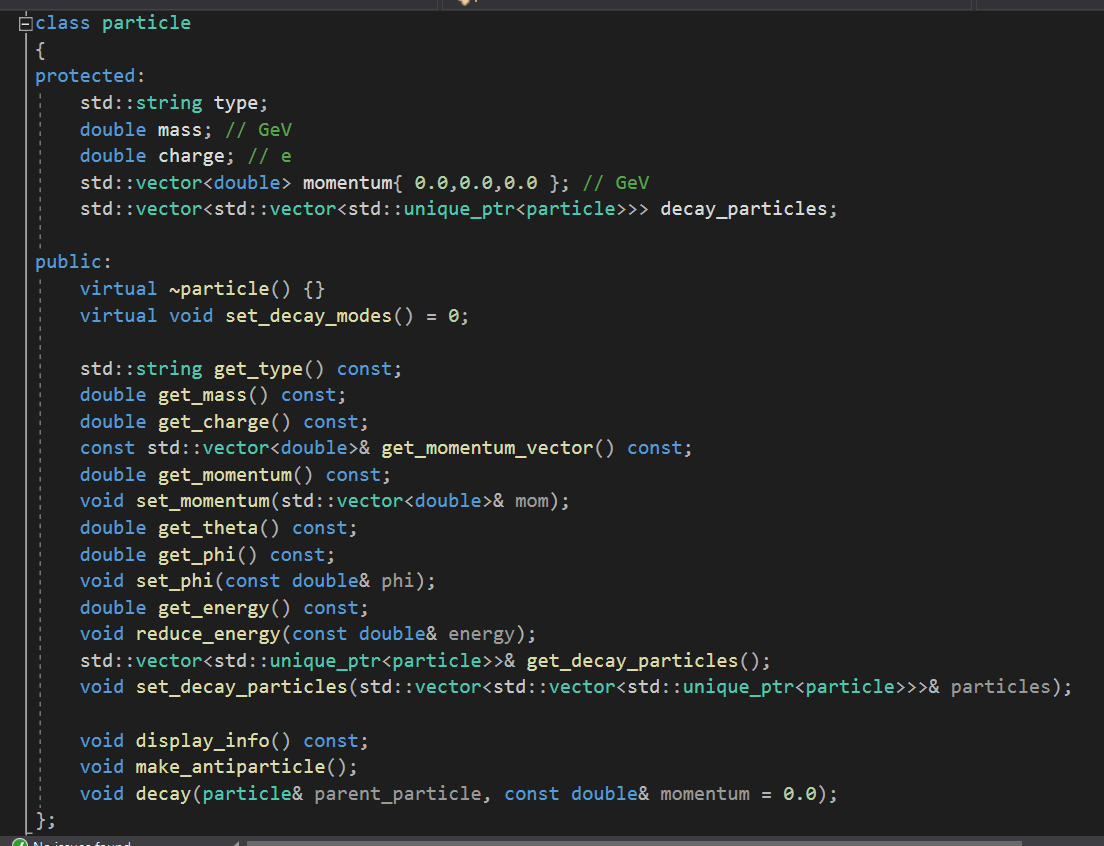
\includegraphics[height=99mm]{snippets/particle.png}
			%\vspace*{-5mm}
			\caption{Class design for particles involved in collisions at the LHC. The mass, momentum and energy of particles are in units of GeV throughout, and the charge in units of the electron charge \textit{e}. The momentum is stored as a \texttt{vector} of the x, y and z components to simplify access in various functions.}
			\label{fig::particle}
		\end{figure}
		
		\justify{
			The abstract derived classes are \texttt{lepton}, \texttt{neutrino} and \texttt{quark}, shown in Figure~\ref{fig::abstractderivedparticles}. The \texttt{charge} is always defined in these classes through their constructors as the charge is common to each of the possible particles in their respective family. The \texttt{neutrino} class also defines the mass and overrides \texttt{particle::set\_decay\_modes()} to an empty function as none of the neutrinos decay. The quarks can be split into two sub-families based on their charge, hence two namespaces, \texttt{up\_type} and \texttt{down\_type}, were used to create two abstract derived \texttt{quark} classes.
		}
			
		\begin{figure}[hbtp]
			\centering
			\begin{tikzpicture}
			\draw (-4.3, 3.5) node[inner sep=0] {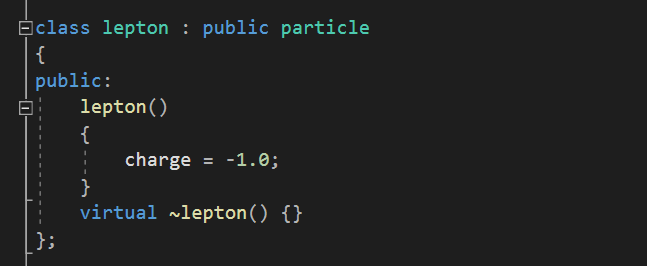
\includegraphics[width=74mm]{snippets/lepton.png}};
			\draw (-4.3, 0.2) node[inner sep=0] {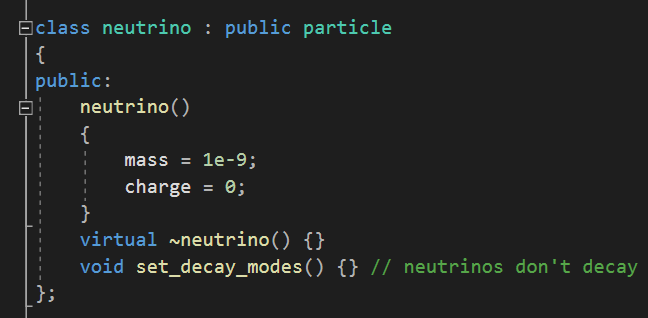
\includegraphics[width=74mm]{snippets/neutrino.png}};
			\draw (3.4, 3.7) node[inner sep=0] {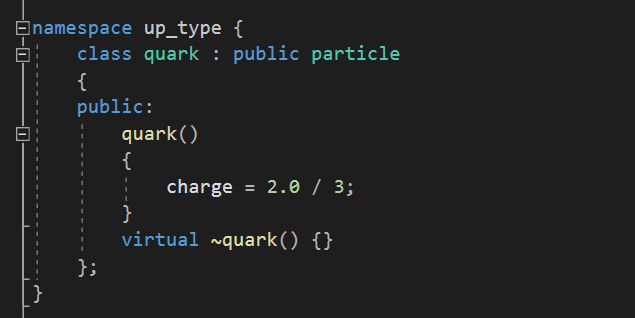
\includegraphics[width=74mm]{snippets/up.png}};
			\draw (3.4, 0) node[inner sep=0] {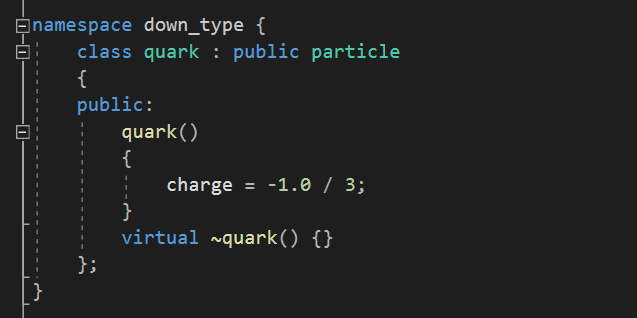
\includegraphics[width=74mm]{snippets/down.png}};
			\end{tikzpicture}
			%\vspace*{-5mm}
			\caption{All of the abstract derived \texttt{particle} classes. The \texttt{charge} is defined in these along with extra definitions for the \texttt{neutrino} class specifically. Namespaces are used to distinguish quarks with positive and negative charge, with the up-type and down-type nomenclature used in particle physics.}
			\label{fig::abstractderivedparticles}
		\end{figure}
		
		\justify{
			Finally, Figure~\ref{fig::muon} shows the derived \texttt{muon} class which inherits from the \texttt{lepton} class. There is a default constructor and a parametrised constructor which takes momentum as an argument. Both constructors have an optional boolean argument, \texttt{is\_antimuon}, which is set by default to \texttt{false}. If \texttt{true} is passed, then the \texttt{particle::make\_antiparticle()} function is called which will change the muons \texttt{charge} and \texttt{type} member data. The constructors and destructor are identical for all other derived \texttt{particle} classes, differing only by what values are passed to the member data and the printed message.
		}
	
		\begin{figure}[hbtp]
			\centering
			\begin{tikzpicture}
			\draw (0, 5.6) node[inner sep=0] {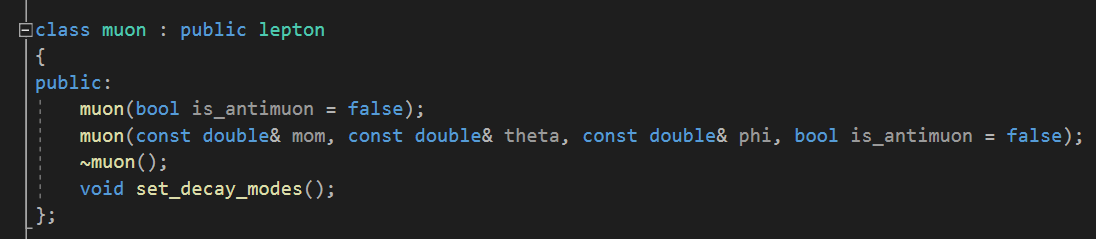
\includegraphics[width=128mm]{snippets/muonh.png}};%24.75mm : 8 lines
			\draw (0, 0) node[inner sep=0] {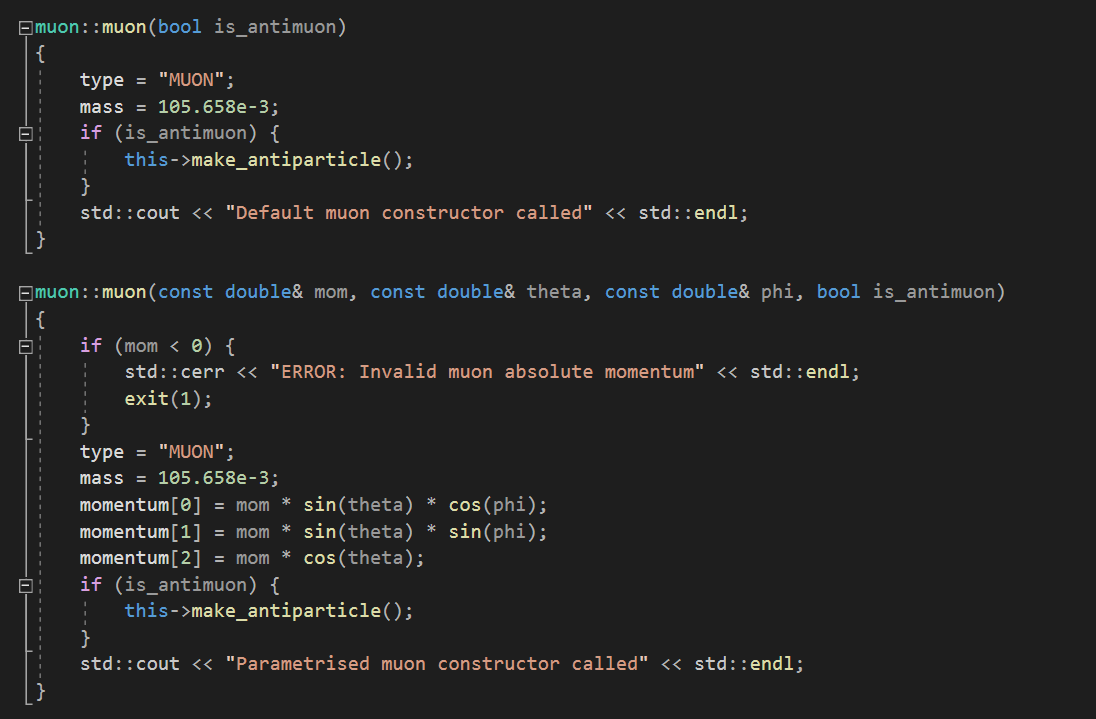
\includegraphics[width=128mm]{snippets/muoncpp.png}};
			\end{tikzpicture}
			%\vspace*{-5mm}
			\caption{Derived \texttt{muon} class with constructor declarations and definitions.}
			\label{fig::muon}
		\end{figure}
		
			\subsubsection{\texttt{particle::set\_decay\_modes()}}
			\label{begin}
			\justify{
				Figure~\ref{fig::set_decay_modes} shows the overridden \texttt{particle::set\_decay\_modes()} function for the \texttt{muon} class. For each possible decay channel, a \texttt{vector} of \texttt{unique\_ptrs} to \texttt{particle} objects is created. Then the relevant objects are pushed onto these \texttt{vectors}, before the \texttt{vectors} themselves are pushed onto \texttt{decay\_particles}. The \texttt{vectors} must be pushed with \texttt{std::move()} as the pointers are unique. The particles which are added to \texttt{decy\_particles} are assumed to be those corresponding to a muon decay rather than an antimuon decay. However, there is then a check on whether the muon is actually an antimuon, in which case all decay particles are set to be antiparticles. Finally, the \texttt{particle::decay()} function is called on the \texttt{particle}.
			}
		
			\begin{figure}[hbtp]
				\centering
				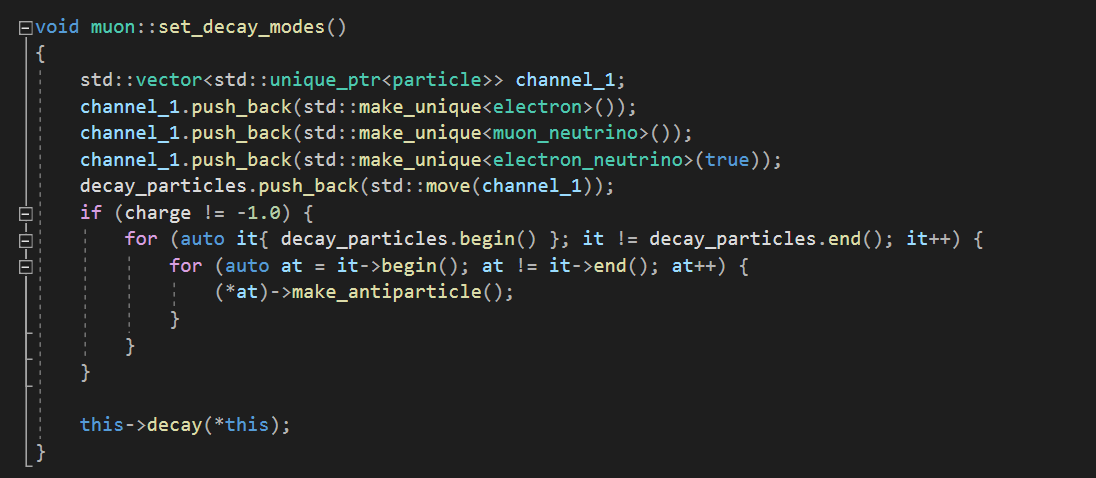
\includegraphics[height=55.7mm]{snippets/setdecaymodes.png}
				%\vspace*{-5mm}
				\caption{Definition of \texttt{particle::set\_decay\_modes()} for the \texttt{muon} class. The muon decays to an electron, emitting a muon-neutrino and an electron-antineutrino.}
				\label{fig::set_decay_modes}
			\end{figure}
		
			\subsubsection{\texttt{particle::decay()}}
			\justify{
				The function first iterates over all channels in \texttt{decay\_particles} and sums the mass of the daughter particles. It checks which channels (if any) have a total daughter mass less than the energy of the parent particle. From those which do, a random channel is selected which the particle will decay via.\\
				In the rest frame of the parent particle, a momentum vector is generated with magnitude $p$, which is half the parent mass, in a random direction $\theta~\epsilon~[0, \pi]$, $\phi~\epsilon~[-\pi, \pi]$. This is then Lorentz boosted back to the lab frame by using the momentum of the parent particle. If the decay channel contains only two particles then a second momentum vector is calculated as the difference between the initial parent momentum and the Lorentz boosted momentum vector. These are then assigned to the decay particles.\\
				Alternatively, if there are more than two decay particles then the Lorentz boosted momentum vector is assigned to the first decay particle. Then a \texttt{recoil} object is instantiated, which inherits from \texttt{particle}. The remaining decay particles are moved onto the \texttt{recoil} using the \texttt{particle::set\_decay\_particles()} function and \texttt{particle::decay()} is called recursively on the \texttt{recoil}. The decay particles, now with altered momenta, are then moved back onto the parent particle and the other channels are removed so that the parent particle has one decay channel with correctly calculated momenta associated with each decay particle.\\
				To be able to calculate the correct Lorentz boost recursively, the parent particle is passed by reference as an argument in \texttt{particle::decay()}. A momentum magnitude is also passed which is used in the calculation of any recoil mass.
			}
		
			\subsubsection{\texttt{particle::get\_theta()}}
			\label{end}
			\justify{
				In the getter function \texttt{particle::get\_theta()}, $\theta$ is found using the z-component of the momentum and the total momentum. There is a chance of dividing by zero if the total momentum is zero, hence error catching was implemented as shown in Figure~\ref{fig::gettheta}. If the momentum is zero then $\theta$ holds no meaning and zero is returned. There is a similar design in the \texttt{particle::get\_phi()} function. 
			}
			
			\begin{figure}[hbtp]
				\centering
				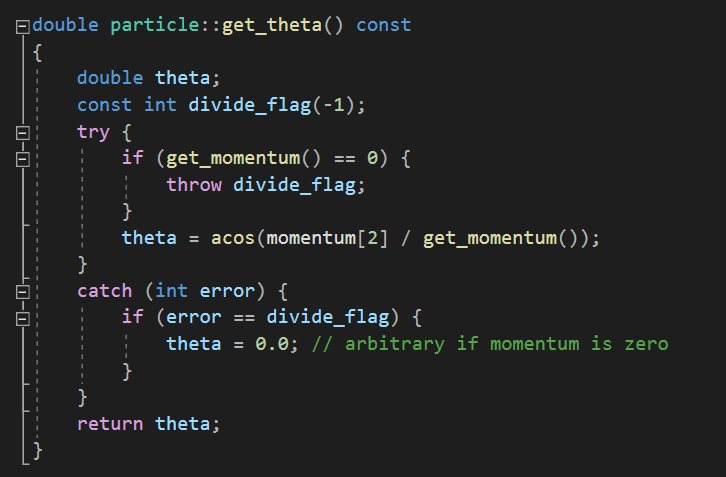
\includegraphics[height=55.7mm]{snippets/gettheta.png}
				%\vspace*{-5mm}
				\caption{Using try-throw-catch to avoid dividing by zero when calculating the polar angle $\theta$ of a momentum vector.}
				\label{fig::gettheta}
			\end{figure}

		\subsection{Detectors}	
		\justify{
			Figure~\ref{fig::detector}(a) shows the \texttt{detector} class design. Each detector segment has a position, size and a \texttt{map} containing particle types and their strength of interaction, if any, with that detector segments medium. The position is stored with a \texttt{const pair} of \texttt{ints} which is used in the \texttt{detector::draw\_detector()} function to display the detector in the console window. Altering the \texttt{centre\_of\_detector} member will move the detector around the console window. The \texttt{detector::draw\_detector()} function also takes a \texttt{COLORREF} argument, which is passed to it from the parametrised \texttt{detector} constructor, so that each detector segment can be coloured differently. An example of a class which inherits from \texttt{detector}, \texttt{e\_calorimeter}, is shown in Figure~\ref{fig::detector}(b). Electrons and photons are solely added to the \texttt{interactions} member of this class so that decays and interactions of \texttt{electron} or \texttt{photon} objects can be triggered when one enters this region of the detector.
		}
		
		\begin{figure}[hbtp]
			\centering
			\begin{tikzpicture}
			\draw (0, 7.8) node[inner sep=0] {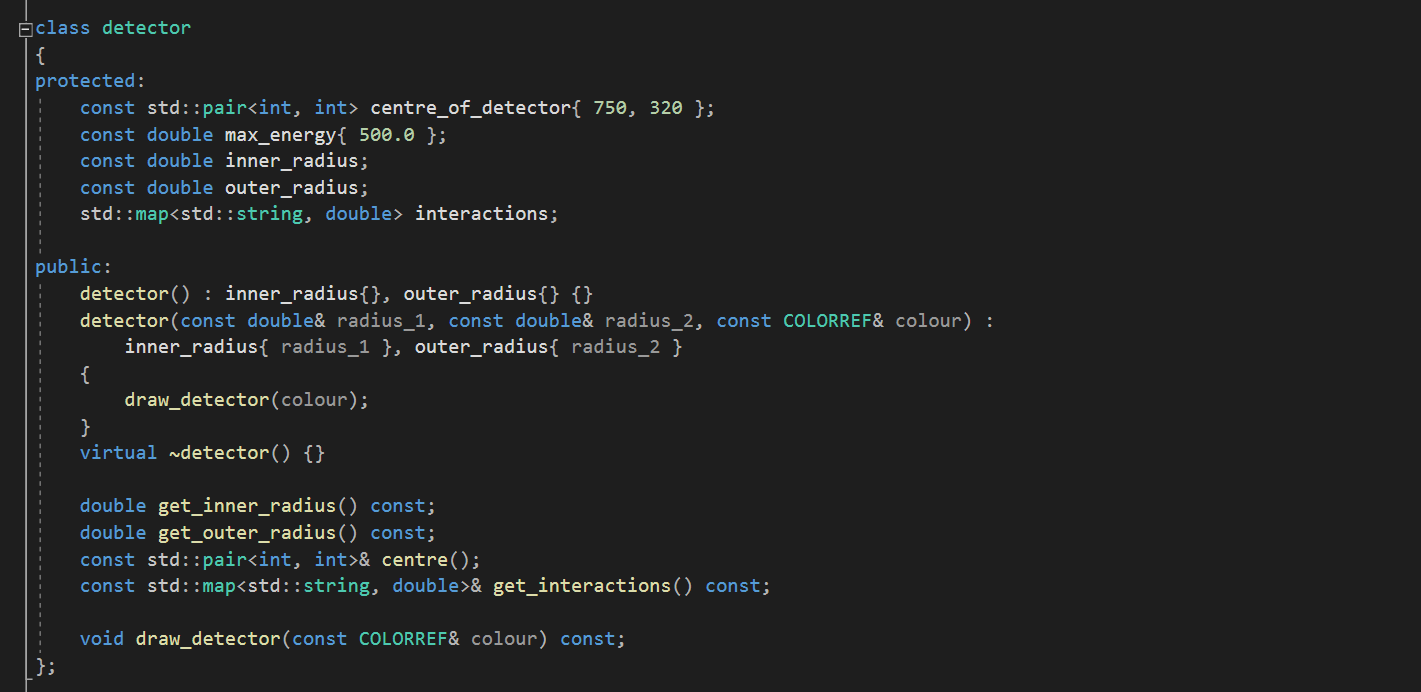
\includegraphics[width=165mm]{snippets/detector.png}};
			\draw (0, 0) node[inner sep=0] {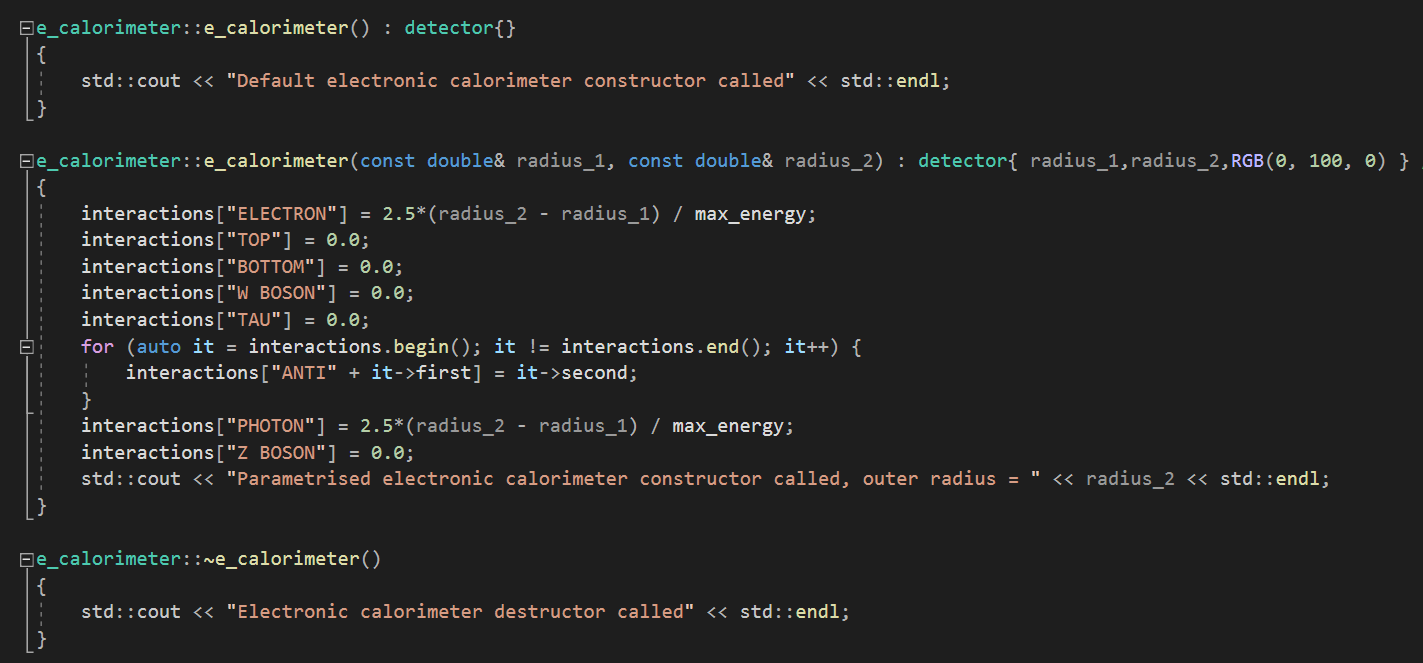
\includegraphics[width=165mm]{snippets/ecal.png}};
			\end{tikzpicture}
			%\vspace*{-5mm}
			\caption{Structure of the \texttt{detector} abstract base class and the implementation of an electronic calorimeter class, \texttt{e\_calorimeter}, which inherits from \texttt{detector}. The only particles which interact with an electronic calorimeter are electrons and photons, hence these are added to \texttt{interactions}.}
			\label{fig::detector}
		\end{figure}
	
		
		\subsection{Collisions}
		\justify{
			The \texttt{collision} class encapsulates the main functionality of the program. As shown in Figure~\ref{fig::collision}, the class contains a polymorphic \texttt{vector} of \texttt{detector} objects. This \texttt{vector} was made \texttt{static} so that all \texttt{collision} instances created during the lifetime of the program have access to the same \texttt{detector} objects. For this to be possible the \texttt{vector} contains \texttt{shared\_ptrs} to the \texttt{detector} objects. The \texttt{static vector} is defined in the collision.cpp file with a set inner and outer radius for each segment. This calls the constructors for the \texttt{detector} segments, each of which call the \texttt{detector::draw\_detetor()} function with a set colour such that the detector is drawn only once at the start of the program and there it remains. The class also contains another polymorphic \texttt{vector} of \texttt{pairs} of \texttt{particle} objects and coordinates, which are represented by a \texttt{pair} of \texttt{ints}.
		}
	
		\begin{figure}[hbtp]
			\centering
			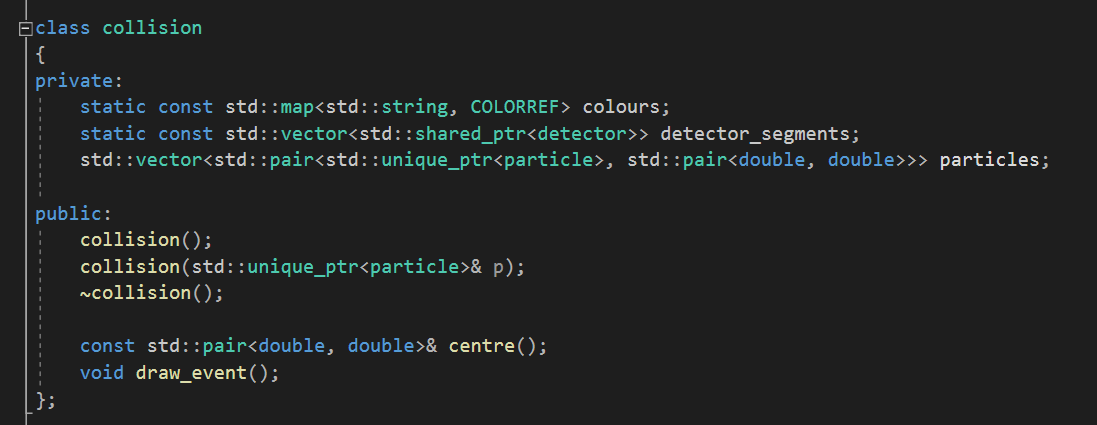
\includegraphics[height=49.5mm]{snippets/collision.png};
			\caption{Class structure of a \texttt{collision} designed to replicate LHC events. The class contains both \texttt{particle} and \texttt{detector} objects.}
			\label{fig::collision}
		\end{figure}
	
		\justify{
			The class has only a default constructor where the \texttt{particles vector} gets filled. The LHC collides protons; the majority of the time it is gluons, up quarks or down quarks which are involved in the interactions. Two partons are drawn at random from these options and, depending on which are drawn, these are interacted in one of a various number of ways. The outgoing particles will include up or down quarks and electroweak bosons. The innermost detector segment, the tracker, then has the weak bosons in its \texttt{interactions map} so that these decay immediately to a range of possible particles.\\
			Figure~\ref{fig::constr} shows an example of one the possible collision outcomes. The colliding partons are quarks which interact via vector boson fusion. Both quarks emit a $Z$ boson which fuse to a single $Z$ boson so that the final state is two quarks + one $Z$ boson. Since the emission of a $Z$ boson is not a defined channel in \texttt{particle::set\_decay\_modes()} for the quarks, the daughter particles are created manually and pushed onto the parent quarks using \texttt{particle::set\_decay\_particles()}. The \texttt{particle::decay()} function is then called on the quarks and a new $Z$ boson is created with a momentum defined as the vector sum of the two daughter $Z$ boson momenta. The particles are then all moved back on to \texttt{particles}.
		}
		
		\begin{figure}[hbtp]
			\centering
			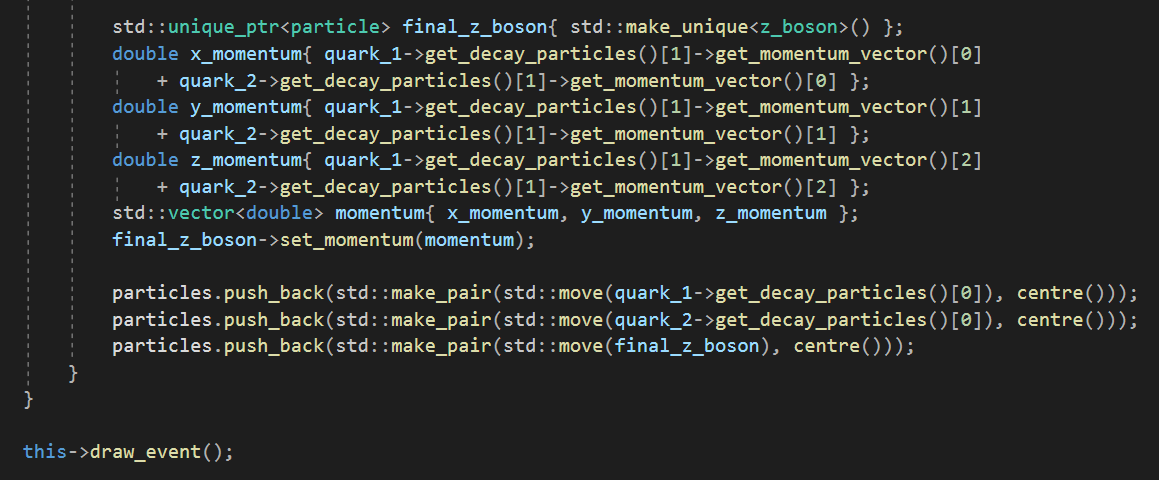
\includegraphics[height=55.7mm]{snippets/constr.png};
			\caption{An example of a type of interaction occurring in proton collisions. If the interacting partons are quarks, vector boson fusion of $Z$'s can occur.}
			\label{fig::constr}
		\end{figure}
	
		\justify{
			When an event is generated, the outgoing \texttt{particle} objects are propagated through the \texttt{detector} segments by the \texttt{collision::draw\_event()} function which is called at the end of the constructor. The function loops over the \texttt{particles} of the \texttt{collision} instance drawing each onto the console window, using the \texttt{momentum} and \texttt{charge} of the \texttt{particle} to propagate it in the correct direction with the correct curvature. This is demonstrated in Figure~\ref{fig::drawevent} where a \texttt{while} loop and the \texttt{SetPixel()} function, which is included in the Windows.h header, are used to draw the path of a particle with non-zero charge. At every step of the propagation, the function finds in which detector segment, if any, the particle is currently located using \texttt{std::find\_if()} and a lambda function. A second lambda function is used with \texttt{std::for\_each()} to check whether the particle interacts with the current detector segment or not, as shown in Figure~\ref{fig::drawevent}. If that is the case, after the particle has traversed more than the interaction distance the \texttt{particle::decay()} function is called on the \texttt{particle} and its daughter particles are pushed onto the \texttt{particles vector} with the coordinates of the current \texttt{particle}.
		}
		
		\begin{figure}[hbtp]
			\centering
			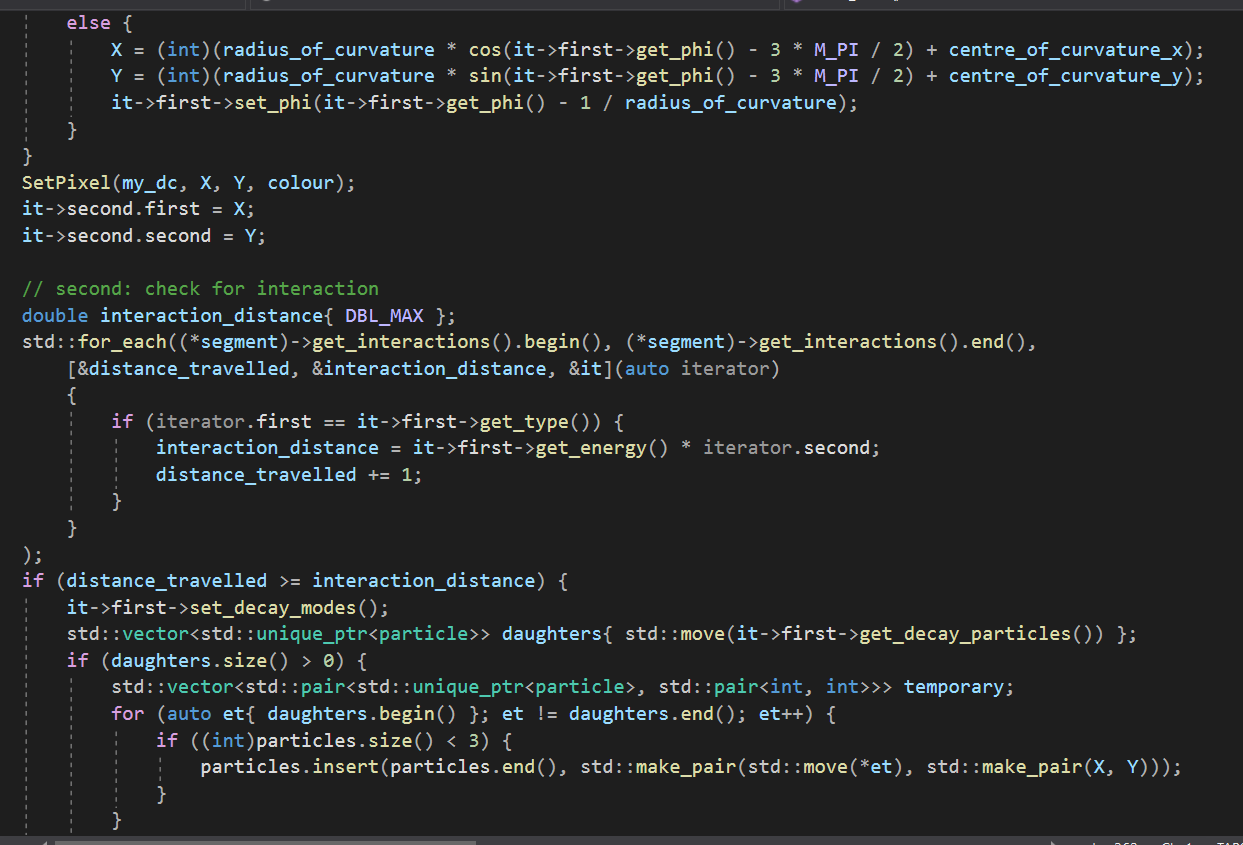
\includegraphics[height=99mm]{snippets/draw.png}
			\caption{A section of the \texttt{collision::draw\_event()} function showing how charged particles are drawn as curves using the \texttt{SetPixel()} function, and how decays in different detector segments are implemented with lambda functions.}
			\label{fig::drawevent}
		\end{figure}
	
		\subsection{Randomness}
		\justify{
			The program often uses random numbers, for example to decide on $\theta$, $\phi$ or on which channel to decay to. The random numbers are required to be of type \texttt{double} or \texttt{int}. Rather than creating a separate random number function for each type, a template function, \texttt{random\_number()} was created which can generate both a \texttt{double} and an \texttt{int}. The function is shown in Figure~\ref{fig::random}; it takes two arguments which control the range in which the random number will be generated. A random integer is drawn in the range [0, 9999] which is then cast to the class type \texttt{T}, meaning that the random number will have a maximum of 4 significant figures. The number is then scaled and transformed to the required range before being returned.
		}
	
		\begin{figure}
			\centering
			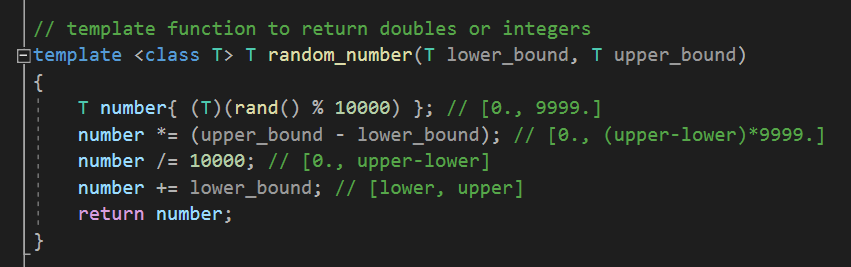
\includegraphics[height=30.9mm]{snippets/random.png}
			\caption{Template function returning a randomly generated \texttt{double} or \texttt{int} in a range specified by the input parameters \texttt{lower\_bound} and \texttt{upper\_bound}. The return value type is governed by the type of input parameters.}
			\label{fig::random}
		\end{figure}
		
	\clearpage
	
	\section{Results}
	\justify{
		Creating one \texttt{collision} object in the \texttt{main()} function gives the result shown in Figure~\ref{fig::output}. A legend is printed in the top left corner so that the user can identify particle types from the track colours and curvature. In this particular example, the initial emerging particles are an $\bar{u}$ quark, a $d$ quark and a $W^{+}$ boson. This will have been the result of two initial gluons; one of which decayed to $d\bar{d}$, and the other to $u\bar{u}$. The $u$ and $\bar{d}$ quarks collide to form the $W^{+}$ boson and the remaining two quarks leave as hadronic jets.\\
		Following the tracks and using the legend, we can work out that the initial $W^{+}$ boson decayed immediately via ${W}^{+}\rightarrow\mu^{+}\nu_{\mu}$, giving the two blue trajectories originating at the centre of the detector. The down quark decayed in the hadronic calorimeter via $d\rightarrow{W}^{-}u$, the $W^{-}$ boson resulting from this going on to decay via $W^{-}\rightarrow\tau\bar{\nu_{\tau}}$ giving one of the green tau neutrino trajectories. The tau then rapidly decayed via $\tau\rightarrow\mu\bar{\nu_{\mu}}\nu_{\tau}$ to give the remaining green tau neutrino track and the other blue muon tracks.\\
		Using the $\mu^{+}$ emitted from the initial $W^{+}$ boson, we can make the assumption that positively charged particles curve clockwise. Then, checking the curvature of the other tracks against the charge of their indicated particle identities, we can verify that decays and particles are produced correctly.
	}
	
	\begin{figure}[hbtp]
		\centering
		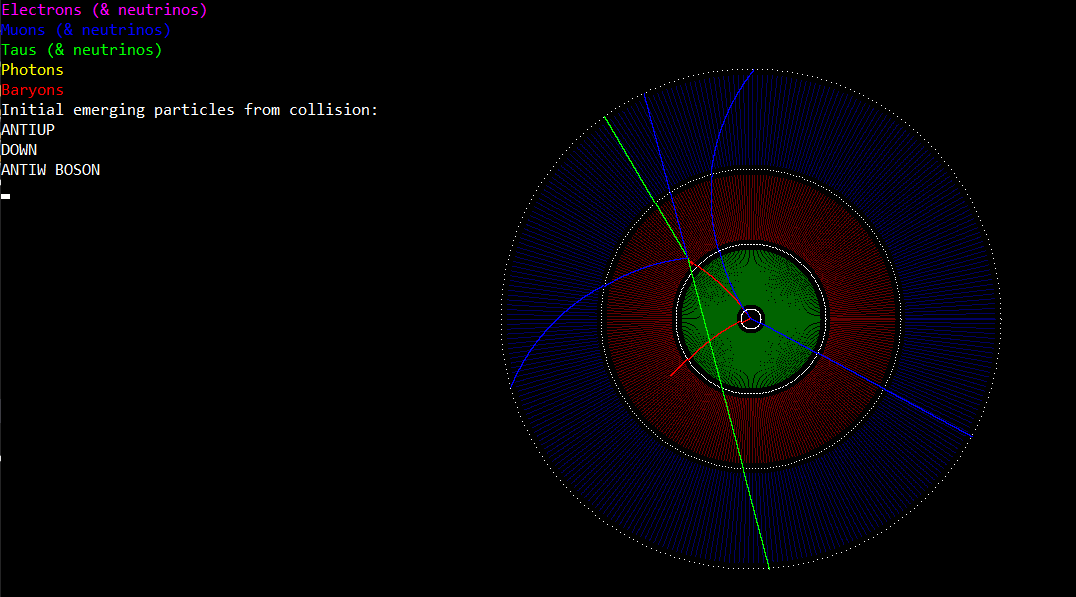
\includegraphics[height=80mm]{snippets/output.png};
		\caption{Example output of one \texttt{collision} instance, showing the drawn detector and particles created from the interaction. On the left is a legend showing the colour each particle type is drawn in as well as a list of the initial particles created in the collision.}
		\label{fig::output}
	\end{figure}
	
	\clearpage
	
	\section{Discussion and conclusion}
	\justify{
		The constructor of the \texttt{collision} class contains a substantial number of lines of code. This is simply due to the number possible interactions which can occur during proton collisions. The constructor could easily be shortened; rather than considering the interactions between a randomly generated pair of colliding partons, the initial emerging particles could be generated with random kinematics from a \texttt{list} containing common initial state particles. This could then include Higgs states, which were not included in the project.\\
		The \texttt{collision::draw\_event()} also contains many lines of code since there are various options for drawing a particular particle's trajectory, for instance its charge and whether or not it interacts with a particular detector medium. To improve on this, functions could be made for charged and non-charged trajectory drawing. The storage of \texttt{particle} objects along with coordinates in a \texttt{vector} of \texttt{pairs} also looks quite messy. Perhaps the coordinates could be moved to be a data member of the particle class instead, further cleaning up the \texttt{collision::draw\_event()} function.\\
		Object-oriented programming in C++ makes for a relatively simple way of managing data necessary to simulate particle events at the LHC. Using run-time polymorphism allows for concise code to iterating over many types of particle and perform the same job on each.
	}
	
	\bibliographystyle{unsrt}
	\bibliography{report}
	
	\clearpage
	
	\appendix
	\appendixpage
	\section{Impact of COVID19 on the work completed and report}
	\justify{
		\textbf{Time lost travelling home:}\\
		At most 2 days of work were lost.\\[1cm]
		\textbf{Lack of access to computers and the internet:}\\
		My laptop supports Visual Studio 2019, however, internet connection at home can be slow at times.\\[1cm]
		\textbf{Limitation in the outcome:}\\
		Not much impact.
	}
	\section{Length}
	\justify{
		The total number of words in this document is 2561.
	}
	
\end{document}